\chapter{Resultados}\label{chapter:results}

\section{}


\begin{figure}
	\centering		
	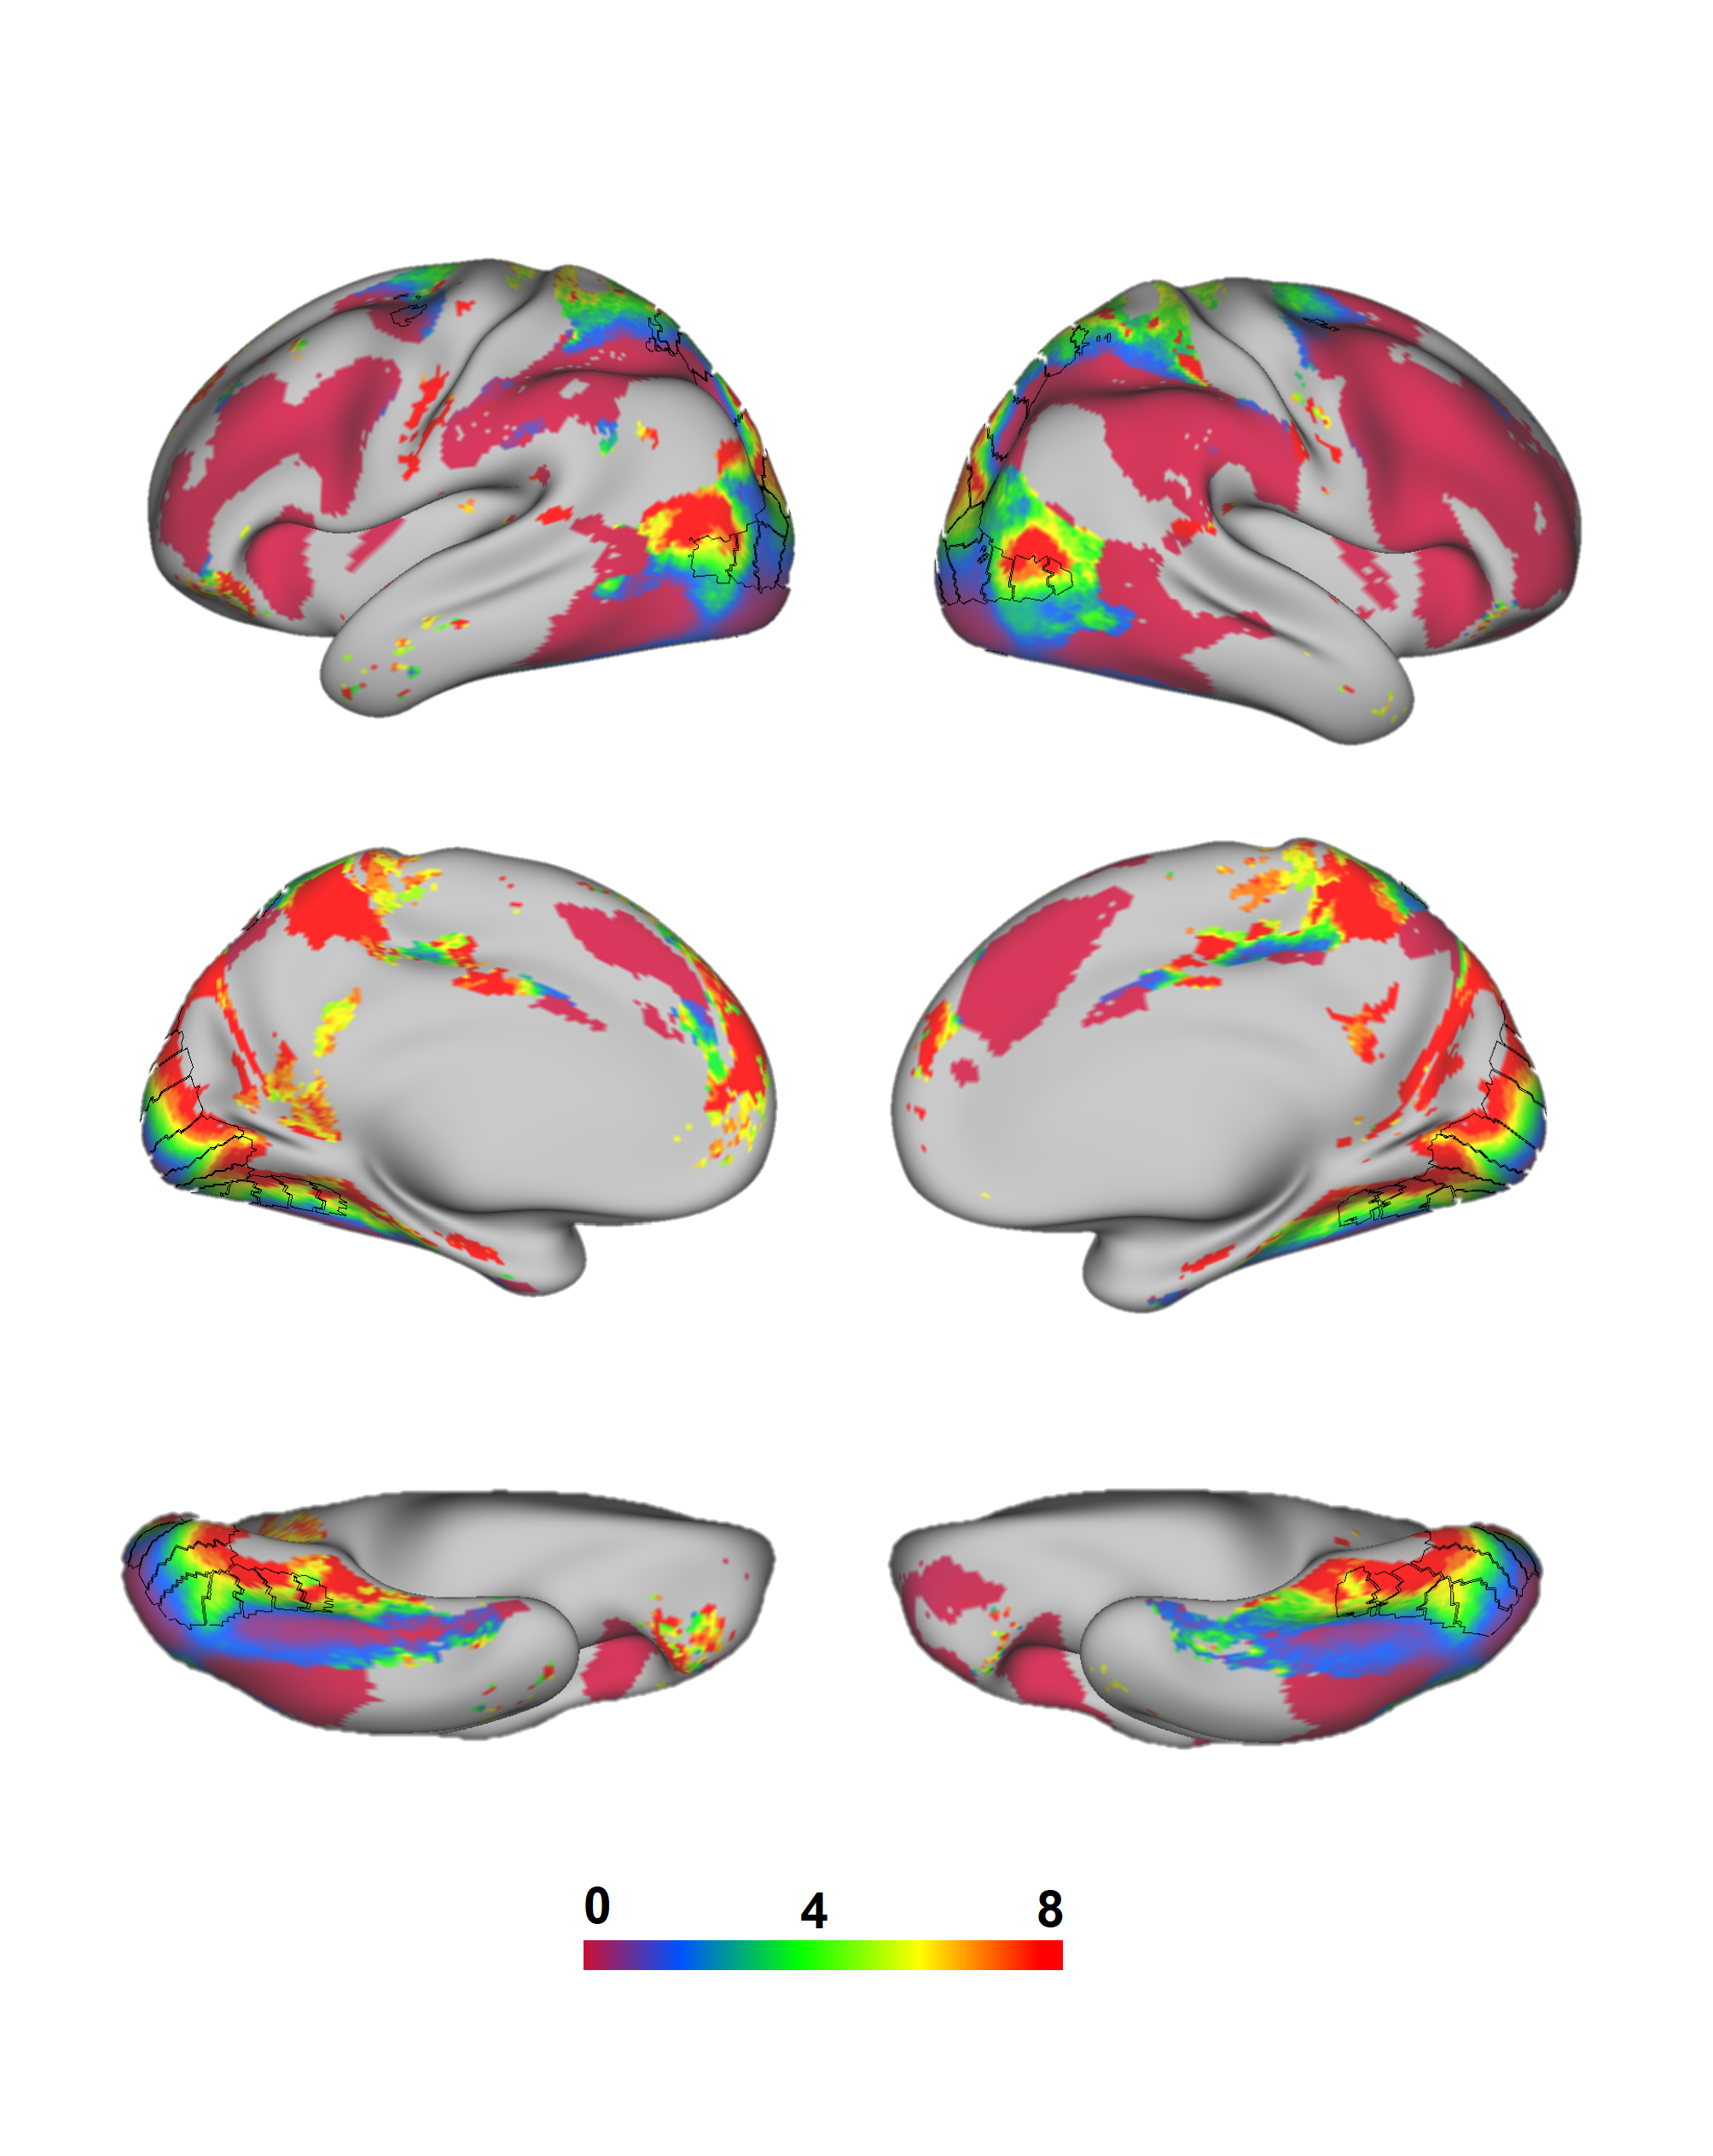
\includegraphics[scale=0.3]{Graphics/brain_eccen}
\end{figure}

- El sigma aumenta con la excentricidad, mayor en areas superiores

- el periodo aumenta con la excentricidad, pendiente aumenta a medida que aumenta areas en la via visual

- destacar relaci\'on en figura \ref{fig:pp_vs_eccen_hem} en \'areas hV4 y VO1 que son las que mayor efecto de lado muestran

- En el modelo lineal mixto que se aplico, se encontr\'o que el efecto de tamano del efecto de los sigma era significativo, comprobandose que el tamano de los pRF en el hemisferio derecho es mayor que en el hemisferio izquierdo.

- Se utiliz\'o un modelo lineal mixto para comprobar el efecto del lado en la preferencia de periodo de los voxels y se concluyo que en \'areas visuales como ... el hemisferio derechos procesa mejor frecuencias espaciales bajas y el hemisferio izquierdo frecuencias espaciales altas.


\begin{figure}
	\centering		
	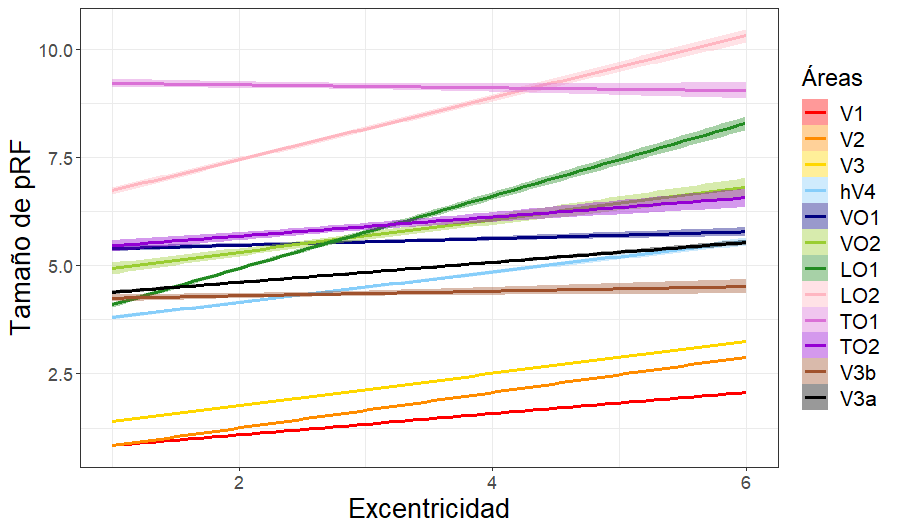
\includegraphics[scale=0.8]{../images/sigma_vs_eccen_all_rois}
	\label{fig:sigma_vs_eccen}
\end{figure}

\begin{figure}
	\centering		
	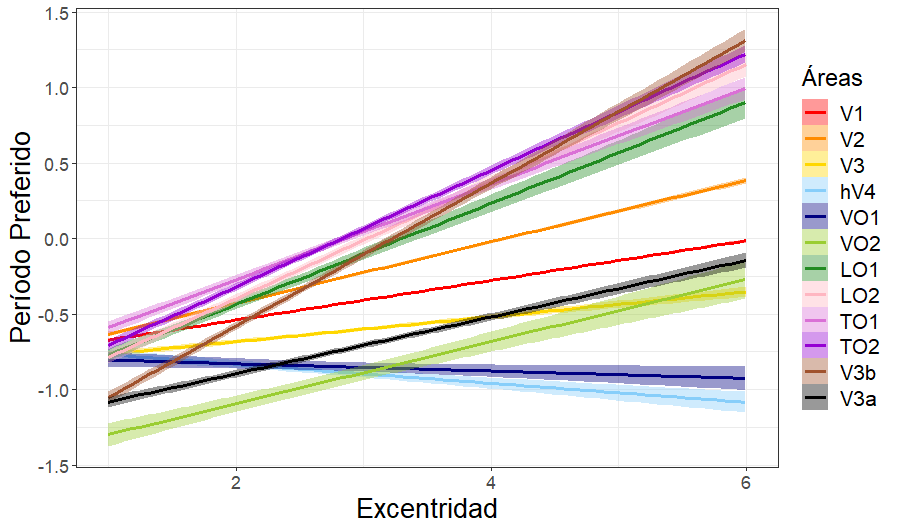
\includegraphics[scale=0.8]{Graphics/pp_vs_eccen_all_rois}
	\label{fig:pp_vs_eccen}
\end{figure}

\begin{figure}
	\centering
	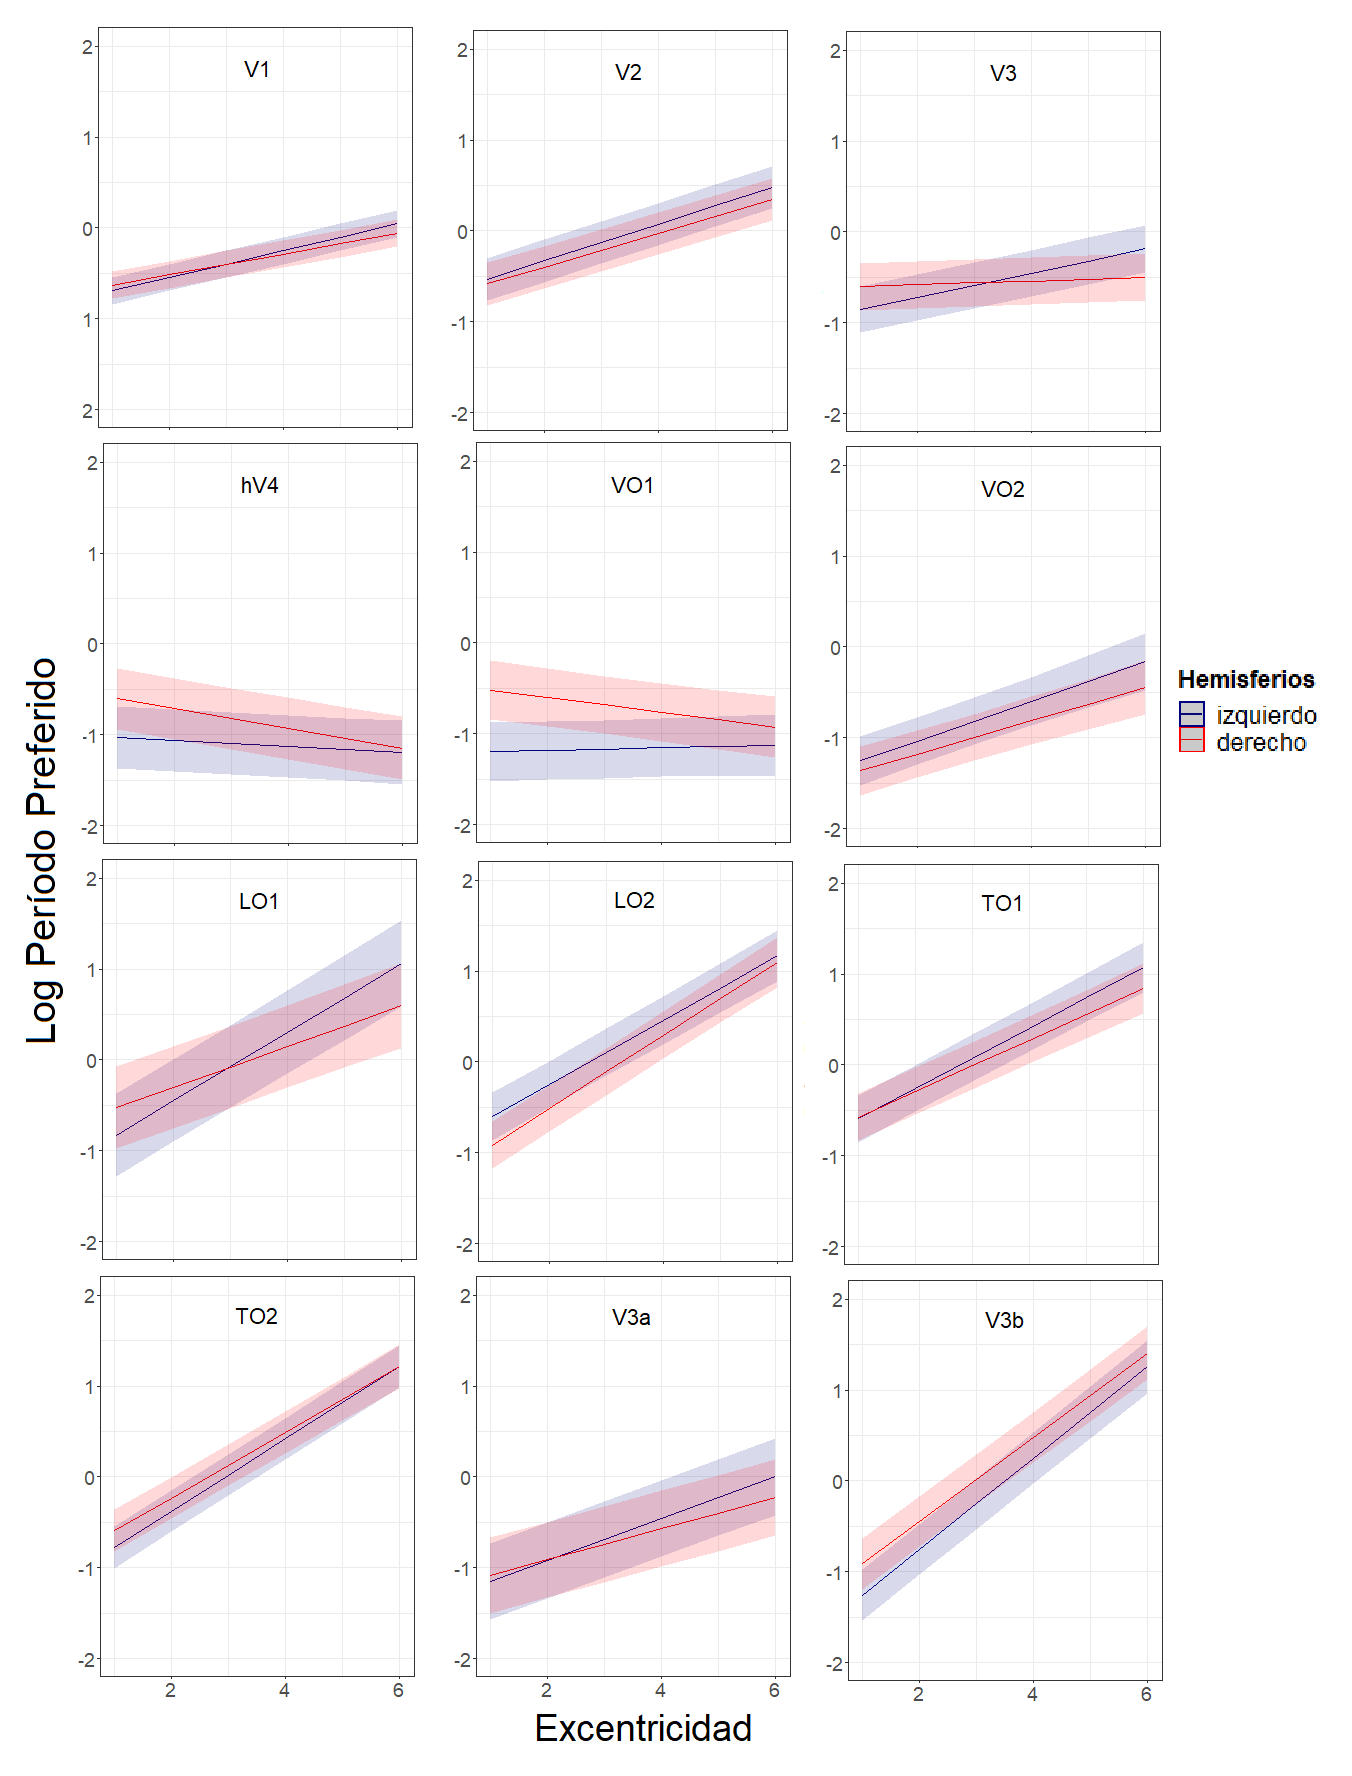
\includegraphics[scale=0.6]{Graphics/compuesto_rois_pp_vs_eccen_hem}
	\label{fig:pp_vs_eccen_hem}
\end{figure}

\begin{figure}
	\centering		
	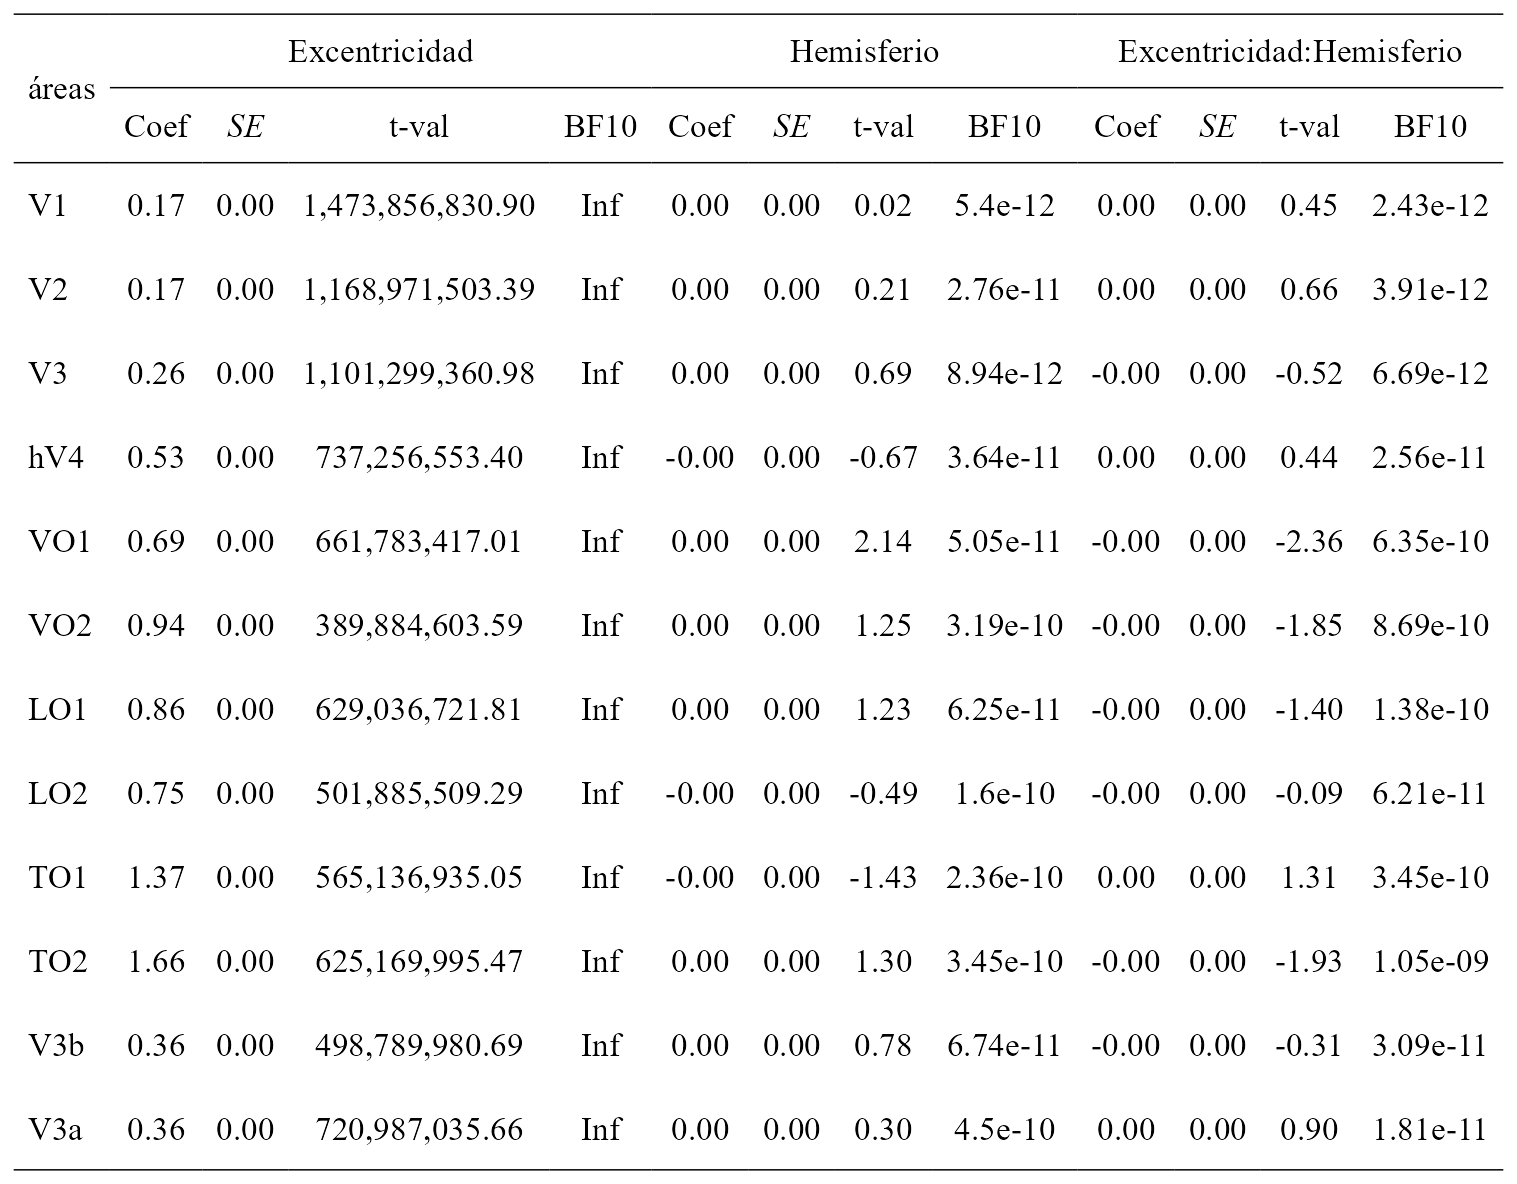
\includegraphics[scale=0.8]{../images/table_sigma}
	\caption{Sigma}
\end{figure}

\begin{figure}
	\centering		
	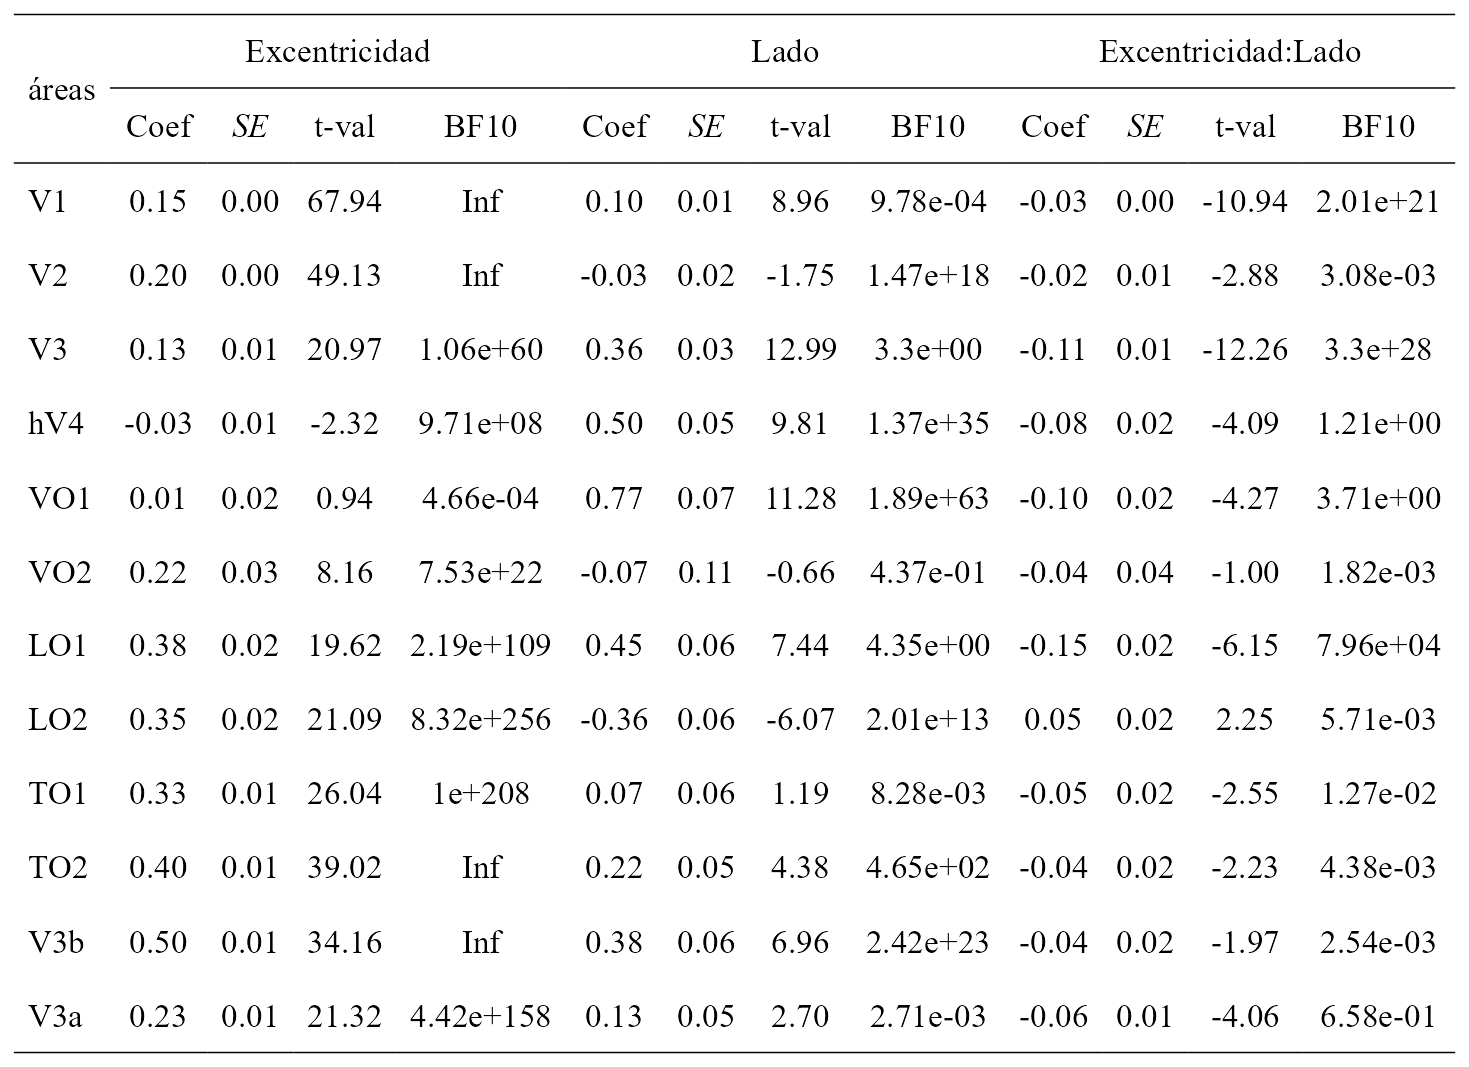
\includegraphics[scale=0.8]{Graphics/table5}
	\caption{PP}
\end{figure}

\begin{figure}
	\centering		
	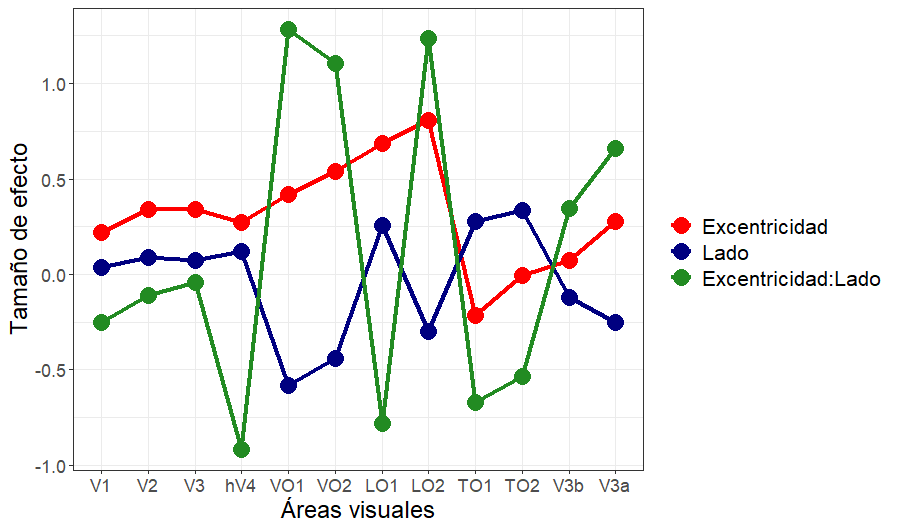
\includegraphics[scale=0.6]{../images/effect_size_eccen_all_rois}
	\caption{sigma}
\end{figure}
\begin{figure}
	\centering		
	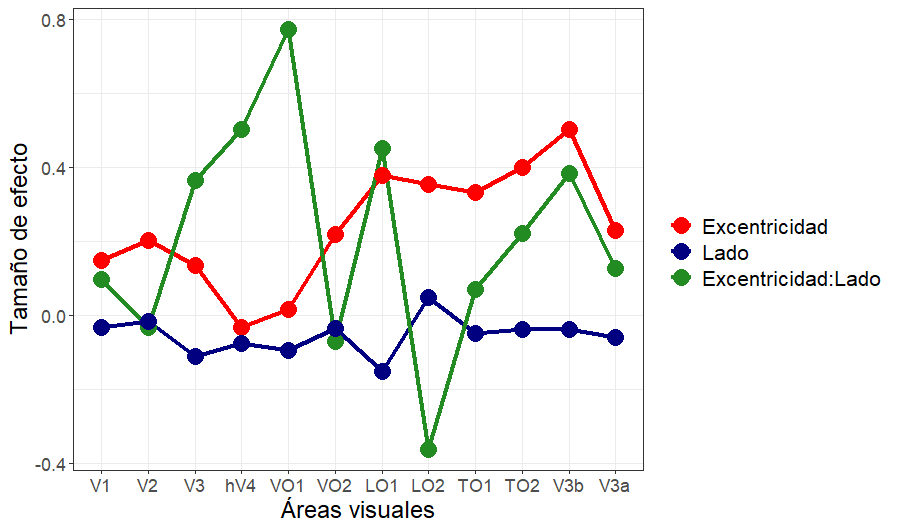
\includegraphics[scale=0.6]{Graphics/effect_size_rois_2}
	\caption{pp}
\end{figure}



